\chapter{Нейросетевой подход}

Нейронная сеть (далее нейросеть) – это математическая модель, а также её программное или аппаратное воплощение, построенная по принципу организации и функционирования биологических нейронных сетей – сетей нервных клеток живого организма \cite{neronnetwork4}. Сегодня такие сети активно используют в практических целях за счет возможности не только разработки, но и обучения. 

Нейросеть для распознавания изображений – это наиболее популярный способ применения нейронной сети \cite{neronnetwork3}.

Три основных компонента нейросети включают в себя \cite{neronnetwork5}:
\begin{itemize}
	\item Входной слой представляет входные данные.
	\item Выходной слой представляет собой выходные данные нейронной сети.
	\item Скрытый слой представляет собой промежуточные узлы, которые делят входное пространство на области с границами. Он принимает набор взвешенных входных данных и производит выходные данные с помощью функции активации.
\end{itemize}

Область применения нейросетей в настоящее время постоянно расширяется, существует множество удачных решений с использованием данного подхода. Столь успешное внедрение нейросетевых решений, прежде всего, обусловлено их преимуществами перед обычными методами\cite{neronnetwork, neronnetwork7}:

\begin{itemize}
	\item Cуществование быстрых алгоритмов обучения, нейронная сеть даже при сотнях входных сигналов и десятках-сотнях тысяч эталонных ситуаций может быть быстро обучена на обычном компьютере;
	\item Возможность работы при наличии большого числа неинформативных, шумовых входных сигналов;
	\item Нейронная сеть одновременно может решать несколько задач на едином наборе входных сигналов;
\end{itemize} 

Несмотря на большие возможности, существует ряд недостатков, которые все же ограничивают применение нейросетевых технологий \cite{neronnetwork8}:
\begin{itemize}
	\item Нейронные сети позволяют найти только субъоптимальное решение, и соответственно неприменимы для задач, в которых требуется высокая точность.
	\item Функционируя по принципу черного ящика, они также неприменимы в случае, когда необходимо объяснить причину принятия решения.
\end{itemize} 

\section {Полносвязные нейросети}

Первая классическая архитектура - полносвязные нейросети. В ней каждый узел (кроме входного и выходного) выступает как входом, так и выходом, образуя скрытый слой нейронов, и каждый нейрон следующего слоя соединён со всеми нейронами предыдущего. Входы подаются с весами, которые в процессе обучения настраиваются и не меняются в последствии. Выходными сигналами сети могут быть все или некоторые выходные сигналы нейронов после нескольких тактов функционирования сети. Все входные сигналы подаются всем нейрона \cite{neronnetwork9}. Это хорошая сеть, так как многие задачи классификации могут быть решены. Однако она не применяется на практике из-за 2 проблем
\begin{itemize}
	\item Много параметров. Например, для сети, у которой на входе картина 100х100, три скрытых слоя по 100 нейтронов каждых, и выходом на 10 классов, число параметров будет больше 1000000.
\end{itemize}

\captionsetup{justification=centering,singlelinecheck=off}
\begin{figure}[h!]
	\centering
	%\begin{center}
		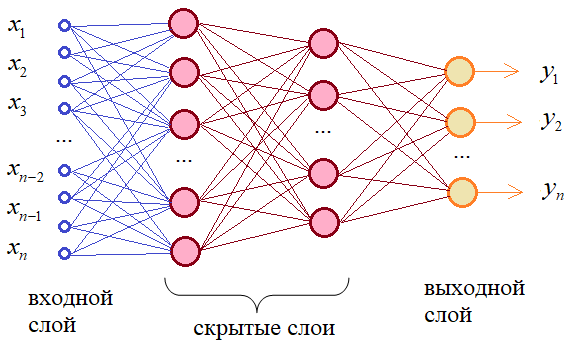
\includegraphics[pages=-, scale=0.9]{img/FNN.png}
		\caption{Метод опорных векторов}  
	%\end{center}
\end{figure}

\section {Свёрточная нейронная сеть}

Свёрточная нейронная сеть (СНC) — это тип модели глубокого обучения для обработки данных, имеющих структуру сетки, например изображений, которая вдохновлена организацией зрительной коры животных \cite{neronnetwork1013, neronnetwork1014} и предназначена для автоматического и адаптивного изучения пространственных иерархий признаков, начиная с низких уровней \cite{neronnetwork10}.

CНC - это математическая конструкция, которая обычно состоит из трех типов слоев (или строительных блоков): свертки, пулинга (подвыборки) и полносвязных слоев. Первые два слоя, свертки и пулинга, выполняют извлечение признаков, тогда как третий, полносвязный слой, отображает извлеченные признаки в конечный результат \cite{neronnetwork10}.

Принцип работы СНC \cite{neronnetwork11}:
\begin{itemize}
	\item В качестве первого слоя всегда выступает сверточный слой. Вводимое изображение представляет матрицу некоторого размера, например 32 х 32 х 3 с пиксельными значениями. Фильтр представляет собой матрицу (её ещё называют матрицей весов или матрицей параметров) размером, например 5 х 5 х 3 и этот фильтр движется по всей области вводного изображения. После прохода фильтра по всей области (движение с шагом один) в итоге получается новая матрица размера 28 х 28 х 1 (можно получить и другую размерность, это зависит от применимости граничных условий при движении фильтра по изображению). Если использовать несколько фильтров размерностью 5 х 5 х 3 вместо одного. Тогда выходным значением будет 28 х 28 х N, где N количество фильтров .
	\item В архитектуре СНС обычно применяется слои пулинга (подвыборки) между последовательности свёрточных слоев. Основная задача состоит в последовательном уменьшении пространственных габаритов (разрешение) изображения с намереньем уменьшения количества входных параметров для следующего слоя и, соответственно, вычислительных операций в сети, а также контроля обучаемости. Слои пулинга работают независимо от глубины данных на входе и масштабируют весь объем пространственно. Среди функций можно выделить функцию максимума и функцию среднего, но также есть и другие.
	\item Последним слоем СНС является полносвязная нейронная сеть. Входными данными для полносвязной нейронной сети являются предыдущие слои и определение свойства, которые больше связаны с определенным классом. Скрытый слой может состоять из нескольких скрытых слоев (обычно два), что позволяет сократить общее количество нейронов в полносвязном слое. Слой полносвязной нейронной сети наблюдают за тем, как высокоуровневые карты свойств сильно связаны с каким-либо классом и содержит конкретные веса, поэтому, когда вычисляются взаимодействие весов с предыдущими слоями, то получаются верные вероятности для разных классов. На выходе получаем N-пространственный вектор, где N соответствует числу классов. Каждое значение в этом N-пространственном векторе представляет собой вероятность конкретного класса \cite{neronnetwork113}.
	\item В итоге СНС в каждом слое преобразования трансформирует данное изображение. Преобразование начинается с первоначальных значений исходного изображения и заканчивается определением класса изображения.
\end{itemize}

\captionsetup{justification=centering,singlelinecheck=off}
\begin{figure}[h!]
	\centering
	%\begin{center}
		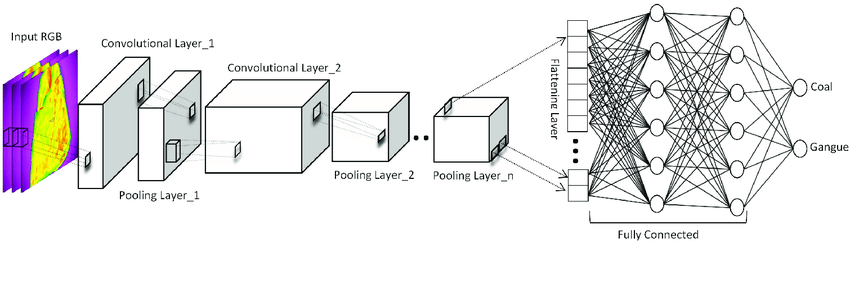
\includegraphics[pages=-, scale=0.5]{img/CNN.png}
		\caption{Метод опорных векторов}  
	%\end{center}
\end{figure}

Основными достоинствами данной сети являются:
\begin{itemize}
	\item В сверточном слое данной сети происходят преобразования изображений, который использует ядра. Его наличие значительно уменьшает время и объем вычислительных ресурсов на обучение \cite{neronnetwork12}.
	\item Использование ядра свертки способствует обобщению полученной информации. Восприятие входного изображения по областям позволяет учесть все его свойства, что увеличивает качество распознавания изображений в несколько раз.
	\item Частичная неизменность к масштабу за счет сжатия изображения.
\end{itemize}

К  сверточной нейронной сети относятся:
\begin{itemize}
	\item Большое количество параметров (количество слоёв, размер ядра свёртки для каждого из слоёв, количество ядер для каждого из слоёв, шаг сдвига и т.д.). Каждый из параметров существенно влияет на результат работы нейронной сети, поэтому для каждой новой задачи они подбираются эмпирически \cite{neronnetwork13}.
	\item Большое количество обучающего материала.
\end{itemize}

\section{Архитектуры нейросетей}

Алгоритмы глубоких нейросетей сегодня обрели большую популярность, которая во многом обеспечивается продуманностью архитектур. Некоторые популярные сегодня архитектуры нейронных сетей: Lenet5, YOLO, ResNet, капсульная нейросеть, ....

\subsection{YOLO}

YOLO — это передовая сеть обнаружения объектов, разработанная Джозефом Редмоном. Главное, что отличает его от других популярных архитектур, — скорость. Модель YOLO действительно быстрая, намного быстрее, чем другие модели. Это означает, что мы можем распознавать объекты в режиме реального времени.

В алгоритме YOLO изображение разделяется на ячейки с использованием сетки. Для каждой ячейки сетки оценивается вероятность присутствия объекта вообще, затем строятся несколько наиболее вероятных положений объекта в виде прямоугольников с центром в данной ячейке, после чего для каждого полученного прямоугольника выполняется оценка вероятностей наличия в нем объектов каждого рассматриваемого класса \cite{neronnetwork13}. На следующем шаге выполняется фильтрация прямоугольников по вероятности нахождения в них объектов. И, наконец, дается класс объекта внутри прямоугольника.

\subsection{Капсульная нейросеть}

Современные виды нейросетей имеют ряд ограничений. Так, нейронная сеть может распознать изображение чашки кофе, но не увидит чашку, перевернутую вверх дном. Точнее – не распознает. Данное ограничение моно изменить с помощью нового подхода «капсульная нейросеть», разработанного доктора Джофри Хинтона с соавторами из Google Brain. Капсульные нейросети не обладают недостатком современных нейронных, которым для обучения требуется огромное число изображений с примерами. Капсулы — небольшие группы виртуальных нейронов — служат для того, чтобы отслеживать различные части предмета, например, нос или ухо кота, и их относительное положение в пространстве. Сеть таких капсул позволит понять, когда на изображении действительно что-то новое, а когда — то же самое, просто под другим углом \cite{neronnetwork14}. 

\section*{Вывод}
Нейронные сети — это метод глубокого обучения, использующий входные изображения, которые могут быть необработанными. Этот подход обладает многими преимуществами, такими как высокая скорость обучения, защита от помех и вход, который решает несколько проблем. Однако никакая причина не может быть названа, чтобы определить результат.

При нейросетевом подход использование только необработанных изображений является большим преимуществом по сравнению с традиционным подходом.